% Provenance (never printed): see sources/outline_sources.md (Year 1:
% geological cross-sections, apparent dip, thickness, boreholes). Every
% Varden Hills number comes from figdata/bachelor-1/varden_sections.py, which
% imports the shared model figdata/shared/region.py; numbers of the exercises
% and problem in the Book 3 scratch calculator and in that script's values.
\chapter{Geologische doorsneden}\label{ch:b1:cross-sections}

Een ingenieursbedrijf plant een tunnel onder de Varden Hills, recht van west naar oost op een
constante hoogte van \qty{200}{m}. Voordat er ook maar één meter wordt geboord, moeten de geologen
zeggen welke gesteenten de machine zal snijden, waar zij de breuk zal kruisen en hoe lang zij in de
kalksteen zal doorbrengen, een gesteente dat open holtes en water kan bevatten. Niemand kan in de
heuvels kijken; maar de \omterm{def:b1:geological-maps:geological-map}{geologische kaart} van \cref{ch:b1:geological-maps}, een paar boringen en de
meetkunde van vlakken zijn genoeg om een verticale snede door de grond te tekenen --- een
doorsnede --- en de antwoorden eruit af te lezen. Dit hoofdstuk leert hoe een doorsnede uit een kaart
wordt opgebouwd, hoe hellingen en diktes veranderen wanneer een snede schuin wordt gelegd, hoe boringen
worden gecorreleerd, en hoe een doorsnede de geschiedenis van de gesteenten vertelt die zij snijdt. Het
eindigt met de tunnel.

\begin{recall}
De oriëntatie van een vlak wordt gegeven door zijn \omterm{def:b1:geological-maps:attitude}{hellingrichting} $\alpha$ en zijn helling
$\delta$, en het vlak door een punt van hoogte $z_0$ in de oorsprong is
$z = z_0 - \tan\delta\,(x\sin\alpha + y\cos\alpha)$; drie punten van een contact bepalen zijn
oriëntatie; de V-regel leest de helling af uit het ontsluitingspatroon in valleien
(\cref{ch:b1:geological-maps}). Een hoogtelijn verbindt punten van gelijke hoogte op een
topografische kaart (Boek 1, klas 9). Jongere gesteenten liggen op oudere, en wat een gesteente
doorsnijdt, is jonger dan dat gesteente (Boek 1, klas 7).
\end{recall}

\section{Van de kaart naar de doorsnede}

\begin{definition}[Geologische doorsnede, topografisch profiel, verticale overdrijving]\label{def:b1:cross-sections:section}
Een \emph{geologische doorsnede}\index{geologische doorsnede} is een tekening van de gesteenteeenheden en
structuren in een verticaal vlak door de grond, langs een lijn die op de kaart is getekend. Haar bovenrand
is het \emph{topografisch profiel}\index{topografisch profiel}, de kromme van de grondhoogte langs de lijn.
De \emph{verticale overdrijving}\index{verticale overdrijving} $e$ van een doorsnede is de verhouding van
haar verticale schaal tot haar horizontale schaal; een doorsnede is \emph{op schaal} wanneer $e = 1$.
\end{definition}

\begin{method}[Een doorsnede uit een kaart opbouwen]\label{met:b1:cross-sections:construct}
\begin{enumerate}
  \item Teken de lijn van de doorsnede op de kaart en leg de rand van een strook papier erlangs; markeer
        waar elke hoogtelijn haar kruist, met haar hoogte, en waar elk contact en elke breuk haar kruist.
  \item Teken een horizontale basislijn van gelijke lengte en een verticale schaal van hoogten (kies $e$,
        en schrijf die op de doorsnede).
  \item Breng elke markering van een hoogtelijn over naar haar hoogte en verbind de punten glad: dit is het
        \omterm{def:b1:cross-sections:section}{topografisch profiel}.
  \item Breng elk contact en elke breuk over naar het profiel, op het punt waar zij de lijn kruisen.
  \item Trek vanaf elk zo'n punt het contact de grond in met zijn helling \emph{in het vlak van de doorsnede}
        --- zijn \omterm{def:b1:cross-sections:apparent-dip}{schijnbare helling} (\cref{sec:b1:cross-sections:apparent}) --- vergroot met $e$ als
        $e \ne 1$; gebruik boringen en \omterm{def:b1:cross-sections:structure-contour}{structuurlijnen} waar die er zijn.
  \item Vul de eenheden tussen de \omterm{def:b1:geological-maps:geological-map}{contacten} aan, met inachtneming van de volgorde van superpositie en van de
        doorsnijdingen, en voeg de legenda, de schalen, de oriëntatie van de lijn en $e$ toe.
\end{enumerate}
\end{method}

\begin{omfigure}
\begin{tikzpicture}[font=\scriptsize, x=1cm, y=1cm]
% map strip with contours crossing the section line
\draw[black!50] (0,2.7) rectangle (9,4.5);
\foreach \x/\h in {0.7/300, 1.6/350, 2.6/400, 4.1/400, 5.0/350, 5.8/300, 7.2/300, 8.2/350} {
  \draw[contour, brown!70!black] (\x-0.25,2.7) .. controls (\x+0.1,3.4) and (\x-0.1,3.8) .. (\x+0.2,4.5);
  \node[brown!60!black, above] at (\x+0.2,4.5) {\h};
}
\draw[omThm, thick] (0,3.6) node[left] {X} -- (9,3.6) node[right] {Y};
\fill[omDef] (3.4,3.6) circle (1.5pt);
\node[omDef, fill=white, inner sep=1pt, above right] at (3.4,3.62) {contact};
% profile
\draw[->] (0,-0.1) -- (0,1.95) node[above] {hoogte (m)};
\draw (0,0) -- (9,0);
\foreach \y/\l in {0/250, 0.5/300, 1.0/350, 1.5/400} { \draw (-0.08,\y) -- (0,\y); \node[left] at (-0.08,\y) {\l}; }
\coordinate (p1) at (0.85,0.5); \coordinate (p2) at (1.75,1.0); \coordinate (p3) at (2.75,1.5);
\coordinate (p4) at (4.25,1.5); \coordinate (p5) at (5.15,1.0); \coordinate (p6) at (5.95,0.5);
\coordinate (p7) at (7.35,0.5); \coordinate (p8) at (8.35,1.0);
\foreach \i/\x in {1/0.85,2/1.75,3/2.75,4/4.25,5/5.15,6/5.95,7/7.35,8/8.35} {
  \draw[black!35, densely dotted] (\x,3.6) -- (p\i);
  \fill (p\i) circle (1.2pt);
}
\draw[thick] (0,0.2) .. controls (0.5,0.3) .. (p1) .. controls (1.3,0.8) .. (p2) .. controls (2.3,1.35) .. (p3)
  .. controls (3.5,1.85) .. (p4) .. controls (4.7,1.25) .. (p5) .. controls (5.5,0.7) .. (p6)
  .. controls (6.6,0.25) .. (p7) .. controls (7.9,0.75) .. (p8) .. controls (8.7,1.15) .. (9,1.2);
\draw[omDef, densely dotted] (3.4,3.6) -- (3.4,1.72);
\draw[omDef, thick] (3.4,1.72) -- (4.45,0.05);
\node[omDef, below right] at (4.3,-0.02) {contact, getekend met zijn schijnbare helling};
\end{tikzpicture}

{\small Een doorsnede bouwen (schematisch): de kruisingen van de hoogtelijnen met de lijn X--Y worden naar
hun hoogten neergezet tot het \omterm{def:b1:cross-sections:section}{topografisch profiel}; een contact dat de lijn kruist, wordt naar het profiel
gebracht en met zijn \omterm{def:b1:cross-sections:apparent-dip}{schijnbare helling} de grond ingetekend.}
\end{omfigure}

De doorsnede hieronder is met de computer gebouwd uit het model van de Varden Hills langs de lijn C--D, die
recht van oost naar west over de kaart loopt op $y = \qty{6}{km}$. Zij toont de \omterm{def:b1:geological-maps:fold}{antiklinaal} waarvan de kern
van zandsteen en fundament verschijnt op $x \approx \qty{3.5}{km}$, de kalksteen en de schalie op haar poten,
het krijt in de \omterm{def:b1:geological-maps:fold}{synklinaal} naar het oosten, en de normale breuk. De tunnellijn, op \qty{200}{m}, en de
boringen B1, B2, B3 van \cref{sec:b1:cross-sections:boreholes} zijn erop getekend.

\begin{omfigure}
\begin{tikzpicture}
\begin{axis}[x=1.4cm, y=0.0042cm, xmin=0, xmax=10, ymin=-500, ymax=650,
  axis on top, tick label style={font=\scriptsize}, label style={font=\small},
  xlabel={afstand oostwaarts vanaf C (km)}, ylabel={hoogte (m)},
  ytick={-400,-200,0,200,400,600}, clip=true]
\addplot[lith schist, draw=black, line width=0.3pt, even odd rule] table {figdata/out/bachelor-1-varden_sections-cd-unit-schist.dat};
\addplot[lith granite, draw=black, line width=0.3pt, even odd rule] table {figdata/out/bachelor-1-varden_sections-cd-unit-granite.dat};
\addplot[om lith={icsTriassic!35}{om sand}, draw=black, line width=0.3pt, even odd rule] table {figdata/out/bachelor-1-varden_sections-cd-unit-sandstone.dat};
\addplot[om lith={icsJurassic!40}{om limestone}, draw=black, line width=0.3pt, even odd rule] table {figdata/out/bachelor-1-varden_sections-cd-unit-limestone.dat};
\addplot[om lith={icsJurassic!15}{om shale}, draw=black, line width=0.3pt, even odd rule] table {figdata/out/bachelor-1-varden_sections-cd-unit-shale.dat};
\addplot[om lith={icsCretaceous!35}{om limestone}, draw=black, line width=0.3pt, even odd rule] table {figdata/out/bachelor-1-varden_sections-cd-unit-chalk.dat};
\addplot[lith alluvium, draw=black, line width=0.3pt, even odd rule] table {figdata/out/bachelor-1-varden_sections-cd-unit-alluvium.dat};
\addplot[black, line width=0.8pt] table {figdata/out/bachelor-1-varden_sections-cd-ground.dat};
\addplot[fault, line width=1.1pt] table {figdata/out/bachelor-1-varden_sections-cd-fault.dat};
\addplot[omThm, line width=1.4pt] coordinates {(1,200) (9,200)};
\node[omThm, font=\scriptsize, fill=white, inner sep=1pt, below] at (axis cs:8.3,190) {tunnel, \qty{200}{m}};
\draw[blue!60!black, line width=0.9pt] (axis cs:1.5,-480) -- (axis cs:1.5,524);
\draw[blue!60!black, line width=0.9pt] (axis cs:3.5,-480) -- (axis cs:3.5,381);
\draw[blue!60!black, line width=0.9pt] (axis cs:5.5,-480) -- (axis cs:5.5,530);
\node[font=\scriptsize, blue!60!black, fill=white, inner sep=1pt] at (axis cs:1.5,-440) {B1};
\node[font=\scriptsize, blue!60!black, fill=white, inner sep=1pt] at (axis cs:3.5,-440) {B2};
\node[font=\scriptsize, blue!60!black, fill=white, inner sep=1pt] at (axis cs:5.5,-440) {B3};
\node[font=\small, above right] at (axis cs:0,650) {C (west)};
\node[font=\small, above left] at (axis cs:10,650) {D (oost)};
\end{axis}
\end{tikzpicture}

\smallskip
\begin{tikzpicture}
\begin{axis}[x=1.4cm, y=0.0014cm, xmin=0, xmax=10, ymin=-500, ymax=650,
  axis on top, tick label style={font=\scriptsize}, ytick={-500,0,500},
  xticklabels={}, clip=true]
\addplot[lith schist, draw=black, line width=0.2pt, even odd rule] table {figdata/out/bachelor-1-varden_sections-cd-unit-schist.dat};
\addplot[lith granite, draw=black, line width=0.2pt, even odd rule] table {figdata/out/bachelor-1-varden_sections-cd-unit-granite.dat};
\addplot[om lith={icsTriassic!35}{om sand}, draw=black, line width=0.2pt, even odd rule] table {figdata/out/bachelor-1-varden_sections-cd-unit-sandstone.dat};
\addplot[om lith={icsJurassic!40}{om limestone}, draw=black, line width=0.2pt, even odd rule] table {figdata/out/bachelor-1-varden_sections-cd-unit-limestone.dat};
\addplot[om lith={icsJurassic!15}{om shale}, draw=black, line width=0.2pt, even odd rule] table {figdata/out/bachelor-1-varden_sections-cd-unit-shale.dat};
\addplot[om lith={icsCretaceous!35}{om limestone}, draw=black, line width=0.2pt, even odd rule] table {figdata/out/bachelor-1-varden_sections-cd-unit-chalk.dat};
\addplot[lith alluvium, draw=black, line width=0.2pt, even odd rule] table {figdata/out/bachelor-1-varden_sections-cd-unit-alluvium.dat};
\addplot[black, line width=0.6pt] table {figdata/out/bachelor-1-varden_sections-cd-ground.dat};
\addplot[fault, line width=0.8pt] table {figdata/out/bachelor-1-varden_sections-cd-fault.dat};
\end{axis}
\end{tikzpicture}

{\small Doorsnede C--D over de Varden Hills, uit het model van de streek. Boven: \omterm{def:b1:cross-sections:section}{verticale overdrijving}
$e = 3$; onder: dezelfde doorsnede op schaal ($e = 1$), waar de poten van \ang{12} zo flauw lijken als zij
zijn. Kleuren als op de \omterm{def:b1:geological-maps:geological-map}{geologische kaart} van \cref{ch:b1:geological-maps}; de breuk (dikke lijn) is de
normale breuk, waarvan het oostelijke blok omlaag is bewogen. De rode lijn is de tunnel van het probleem;
B1--B3 zijn boringen.}
\end{omfigure}

\omterm{def:b1:cross-sections:section}{Verticale overdrijving} maakt dunne eenheden en flauw reliëf leesbaar, maar zij vervormt elke hoek: de
poten van \ang{12} van de \omterm{def:b1:geological-maps:fold}{plooi} lijken in de bovenste doorsnede ongeveer \ang{32} te zijn. De volgende
paragraaf zegt precies hoe.

\section{Schijnbare helling}\label{sec:b1:cross-sections:apparent}

\begin{definition}[Schijnbare helling]\label{def:b1:cross-sections:apparent-dip}
De \emph{schijnbare helling}\index{schijnbare helling} $\beta$ van een vlak in een gegeven verticale doorsnede
is de hoek tussen de horizontale en het spoor van het vlak in die doorsnede. Zij is gelijk aan de ware helling
$\delta$ wanneer de doorsnede langs de \omterm{def:b1:geological-maps:attitude}{hellingrichting} loopt, en nul wanneer zij langs de \omterm{def:b1:geological-maps:attitude}{strijk} loopt.
\end{definition}

\begin{theorem}[Schijnbare helling]\label{thm:b1:cross-sections:apparent-dip}
Een vlak met helling $\delta$ en \omterm{def:b1:geological-maps:attitude}{hellingrichting} $\alpha$, gesneden door een verticale doorsnede met \omterm{def:b1:spherical-astronomy:horizontal}{azimut}
$\theta$, toont de \omterm{def:b1:cross-sections:apparent-dip}{schijnbare helling} $\beta$ met
\[
  \tan\beta = \tan\delta\,\cos\gamma, \qquad \gamma = \alpha - \theta ,
\]
waarbij het vlak in de richting $\theta$ daalt wanneer $\cos\gamma > 0$.
In het bijzonder is $|\beta| \le \delta$, met gelijkheid alleen langs de \omterm{def:b1:geological-maps:attitude}{hellingrichting}.
\end{theorem}

\begin{proof}
Neem het vlak $z = z_0 - \tan\delta\,(x\sin\alpha + y\cos\alpha)$ van
\cref{ch:b1:geological-maps}. Langs de doorsnede is een horizontale stap van lengte
$s$ in de richting $\theta$ gelijk aan $(x, y) = s(\sin\theta, \cos\theta)$, dus
$z = z_0 - s\tan\delta\,(\sin\theta\sin\alpha + \cos\theta\cos\alpha) =
z_0 - s\tan\delta\cos(\alpha - \theta)$. Het spoor is een rechte lijn die daalt met
$\tan\delta\cos\gamma$ per eenheid horizontale afstand: dat is $\tan\beta$. Omdat
$|\cos\gamma| \le 1$, geldt $|\tan\beta| \le \tan\delta$.
\end{proof}

\begin{omfigure}
\begin{tikzpicture}[font=\scriptsize, x={(1cm,0cm)}, y={(0.6cm,0.45cm)}, z={(0cm,1cm)}]
% hidden edges of the block
\draw[black!30, densely dashed] (0,0,0) -- (0,3,0) -- (4,3,0);
\draw[black!30, densely dashed] (0,3,0) -- (0,3,2);
% the oblique vertical section, from the front-left corner to the back-right one
\fill[black!10, opacity=0.7] (0,0,0) -- (4,3,0) -- (4,3,2) -- (0,0,2) -- cycle;
\draw[black!45] (0,0,0) -- (4,3,0) -- (4,3,2);
% the dipping plane, from the top-west edge down to the base
\fill[omDef!25, opacity=0.75] (0,0,2) -- (2.6,0,0) -- (2.6,3,0) -- (0,3,2) -- cycle;
\draw[omDef] (2.6,0,0) -- (2.6,3,0);
\draw[omDef, very thick] (0,0,2) -- (2.6,0,0);
\draw[omThm, very thick] (0,0,2) -- (2.6,1.95,0);
% visible edges of the block
\draw[black!70] (0,0,0) -- (4,0,0) -- (4,0,2) -- (0,0,2) -- cycle;
\draw[black!70] (0,0,2) -- (0,3,2) -- (4,3,2) -- (4,0,2);
\draw[black!70] (4,0,0) -- (4,3,0) -- (4,3,2);
% labels
\draw[omDef] (2.0,0,0) arc[start angle=180, end angle=142.4, radius=0.6cm];
\node[omDef] at (1.7,0,0.2) {$\delta$};
\node[omDef, below, align=center] at (1.3,0,0) {voorvlak, langs de hellingrichting:\\ ware helling $\delta$};
\node[omThm, right, align=left] at (4.45,2.2,0.3) {schuine doorsnede (grijs):\\ schijnbare helling $\beta < \delta$};
\node[above] at (0,1.5,2) {N};
\draw[->] (0.15,1.5,2.05) -- (0.15,2.2,2.05);
\end{tikzpicture}

{\small \omterm{def:b1:cross-sections:apparent-dip}{Schijnbare helling} (schematisch blok). Een vlak dat naar het oosten helt (blauw) toont zijn ware
helling $\delta$ op het voorvlak, een verticaal vlak langs de \omterm{def:b1:geological-maps:attitude}{hellingrichting}; op de grijze verticale
doorsnede, schuin gesneden, daalt zijn spoor (rood) flauwer, met de \omterm{def:b1:cross-sections:apparent-dip}{schijnbare helling} $\beta$; op een doorsnede
langs de \omterm{def:b1:geological-maps:attitude}{strijk}, noord--zuid, zou het horizontaal zijn.}
\end{omfigure}

\begin{proposition}[Hoeken in een overdreven doorsnede]\label{prop:b1:cross-sections:exaggeration}
In een doorsnede getekend met \omterm{def:b1:cross-sections:section}{verticale overdrijving} $e$ wordt een lijn met \omterm{def:b1:cross-sections:apparent-dip}{schijnbare helling} $\beta$
getekend onder de hoek $\beta'$ met $\tan\beta' = e\tan\beta$.
\end{proposition}

\begin{proof}
Over een horizontale afstand $s$ daalt de lijn met $s\tan\beta$; getekend met een verticale schaal $e$ maal de
horizontale schaal, verschijnt de daling als $es\tan\beta$ over dezelfde getekende lengte $s$.
\end{proof}

\begin{example}
De oostflank van de \omterm{def:b1:geological-maps:fold}{antiklinaal} van Varden helt \ang{12.16} naar \ang{080.7}
(\cref{ch:b1:geological-maps}). In de oost--west doorsnede C--D is
$\gamma = \ang{80.7} - \ang{90} = \ang{-9.3}$, en $\tan\beta =
\tan\ang{12.16}\cos\ang{9.3} = 0.2154\times0.9868 = 0.2126$: $\beta =
\ang{12.0}$. Getekend met $e = 3$ verschijnt zij onder $\arctan(3\times0.2126) =
\ang{32.5}$. In de doorsnede A--B met \omterm{def:b1:spherical-astronomy:horizontal}{azimut} \ang{071.6} is $\gamma = \ang{9.1}$
en $\beta = \ang{12.0}$ eveneens: beide doorsneden lopen dicht bij de \omterm{def:b1:geological-maps:attitude}{hellingrichting}. De breuk, die
\ang{60} naar \ang{120} helt, heeft in C--D de \omterm{def:b1:cross-sections:apparent-dip}{schijnbare helling}
$\arctan(\tan\ang{60}\cos\ang{30}) = \arctan 1.5 = \ang{56.3}$.
\end{example}

\section{Dikte}

\begin{definition}[Ware dikte, verticale dikte]\label{def:b1:cross-sections:thickness}
De \emph{ware dikte}\index{ware dikte} $t$ van een laag is de afstand tussen haar basis en haar top, loodrecht
op de gelaagdheid gemeten. Haar \emph{verticale dikte}\index{verticale dikte} $h$ is dezelfde afstand, gemeten langs
de verticale, zoals een verticale boring haar snijdt.
\end{definition}

\begin{proposition}[Dikte van een hellende laag]\label{prop:b1:cross-sections:thickness}
Voor een laag met helling $\delta$:
\begin{enumerate}
  \item $t = h\cos\delta$;
  \item op horizontaal terrein, als de \omterm{def:b1:geological-maps:geological-map}{ontsluiting} van de laag de breedte $w$ heeft, gemeten loodrecht op de
        \omterm{def:b1:geological-maps:attitude}{strijk}, geldt $t = w\sin\delta$;
  \item op terrein dat onder de hoek $\sigma$ helt in de richting loodrecht op de \omterm{def:b1:geological-maps:attitude}{strijk}, met $w$ langs het
        terrein gemeten, geldt $t = w\sin(\delta + \sigma)$ als het terrein tegengesteld aan de helling helt, en
        $t = w\sin(\delta - \sigma)$ als het in dezelfde richting maar minder steil helt dan de lagen.
\end{enumerate}
\end{proposition}

\begin{proof}
In het verticale vlak loodrecht op de \omterm{def:b1:geological-maps:attitude}{strijk} zijn de basis en de top van de laag twee evenwijdige lijnen die
onder $\delta$ helling hebben, op een afstand $t$. (1) Een verticaal lijnstuk dat ze verbindt, maakt de hoek
$\delta$ met hun gemeenschappelijke normaal, dus $t = h\cos\delta$. (2)--(3) Een lijnstuk van lengte $w$ dat ze
langs het terrein verbindt, maakt met de gelaagdheid de hoek $\delta$ wanneer het terrein vlak is, $\delta + \sigma$
wanneer het terrein naar de \omterm{def:b1:geological-maps:attitude}{hellingrichting} toe stijgt (de twee hellingen tellen op), en $\delta - \sigma$ wanneer
het in dezelfde richting daalt; de afstand tussen de evenwijdige lijnen is de lengte van het lijnstuk maal de sinus
van die hoek.
\end{proof}

\begin{omfigure}
\begin{tikzpicture}[font=\scriptsize]
\pgfmathsetmacro{\d}{25}\pgfmathsetmacro{\t}{1.3}
\pgfmathsetmacro{\h}{\t/cos(\d)}\pgfmathsetmacro{\w}{\t/sin(\d)}
\pgfmathsetmacro{\X}{4.0}
\fill[icsJurassic!30] (-\w,0) -- (0,0) -- (\X,{-\X*tan(\d)}) -- (\X,{-\X*tan(\d)-\h}) -- cycle;
\draw[thick] (0,0) -- (\X,{-\X*tan(\d)}) node[right] {top van de laag};
\draw[thick] (-\w,0) -- (\X,{-\X*tan(\d)-\h}) node[right] {basis};
\draw[black!70] ({-\w-0.8},0) -- (\X+0.6,0) node[right] {vlak terrein};
% vertical thickness
\draw[omThm, thick, <->] (1.0,{-1.0*tan(\d)}) -- (1.0,{-1.0*tan(\d)-\h});
\node[omThm, right] at (1.0,{-1.0*tan(\d)-0.55*\h}) {$h$};
% true thickness, perpendicular to the bedding
\coordinate (A) at (2.8,{-2.8*tan(\d)});
\draw[omDef, thick, <->] (A) -- ++({-90-\d}:\t);
\node[omDef, right] at ($(A)+({-90-\d}:0.5*\t)$) {$t$};
% outcrop width on flat ground
\draw[black, thick, <->] (-\w,0.2) -- (0,0.2);
\node[above] at ({-0.5*\w},0.2) {$w$};
\draw[omThm] (1.0,0) arc[start angle=0, end angle=-\d, radius=1.0];
\node[omThm] at (1.25,-0.22) {$\delta$};
\end{tikzpicture}

{\small Diktes van een hellende laag in het verticale vlak loodrecht op de \omterm{def:b1:geological-maps:attitude}{strijk}: de \omterm{def:b1:cross-sections:thickness}{ware dikte} $t$, loodrecht op
de gelaagdheid; de \omterm{def:b1:cross-sections:thickness}{verticale dikte} $h = t/\cos\delta$; de breedte van de \omterm{def:b1:geological-maps:geological-map}{ontsluiting} $w = t/\sin\delta$ op vlak terrein
(schematisch, met $\delta = \ang{25}$).}
\end{omfigure}

In de Varden Hills snijdt een boring die van boven in de kalksteen komt, de kalksteen over \qty{180}{m} kern: dat is haar \omterm{def:b1:cross-sections:thickness}{verticale dikte}. Haar \omterm{def:b1:cross-sections:thickness}{ware
dikte} is $180\cos\ang{12.16} = \qty{176.0}{m}$. Een dunne en een dikke eenheid kunnen dezelfde ontsluitingsbreedte
tonen als hun hellingen verschillen, en een steile laag kan een brede \omterm{def:b1:geological-maps:geological-map}{ontsluiting} tonen op een helling die met
haar meeloopt: de dikte wordt nooit rechtstreeks uit een kaart afgelezen.

\section{Boringen en structuurlijnen}\label{sec:b1:cross-sections:boreholes}

\begin{definition}[Boorstaat, correlatie]\label{def:b1:cross-sections:log}
Een \emph{boorstaat}\index{boorstaat} is de registratie, tegen de diepte, van de gesteenten die een boring
aantreft: de eenheden, de diepten van hun \omterm{def:b1:geological-maps:geological-map}{contacten} en elke gemeten eigenschap. \emph{Correlatie}\index{correlatie (van boorstaten)}
is het aan elkaar koppelen van dezelfde eenheden en \omterm{def:b1:geological-maps:geological-map}{contacten} van de ene staat naar de andere.
\end{definition}

Drie boringen op de lijn C--D geven de volgende diepten onder het maaiveld van de basis van elke eenheid (een
streepje: het contact ligt boven het maaiveld, geërodeerd):
\begin{center}
\small
\begin{tabular}{lcccccc}
\hline
boring & $x$ (km) & maaiveld (m) & krijt & schalie & kalksteen & zandsteen \\
\hline
B1 & 1.5 & 524.02 & 388.98 & 488.98 & 668.98 & 788.98 \\
B2 & 3.5 & 380.64 & --- & --- & 100.48 & 220.48 \\
B3 & 5.5 & 529.98 & 394.93 & 494.93 & 674.93 & 794.93 \\
\hline
\end{tabular}
\end{center}
B2 begint in de kalksteen, op de kruin van de \omterm{def:b1:geological-maps:fold}{antiklinaal}; B1 en B3 beginnen in het krijt, op de poten. Door de
diepten van de grondhoogte af te trekken, krijgt men de hoogten van de \omterm{def:b1:geological-maps:geological-map}{contacten}: de basis van de kalksteen ligt in
B2 op $380.64 - 100.48 = \qty{280.16}{m}$ en in B3 op $529.98 - 674.93 =
\qty{-144.95}{m}$, \qty{425.11}{m} lager over \qty{2}{km}, een helling van \num{0.2126}: de \omterm{def:b1:cross-sections:apparent-dip}{schijnbare helling} van
\ang{12.0} die hierboven is gevonden. De \omterm{def:b1:cross-sections:log}{boorstaat} van B1 en die van B3 geven dezelfde diktes, \qty{100}{m} schalie, \qty{180}{m} kalksteen en
\qty{120}{m} zandsteen: de eenheden hebben dezelfde \omterm{def:b1:cross-sections:thickness}{verticale dikte} op beide poten.

\begin{omfigure}
\begin{tikzpicture}[font=\scriptsize, x=1cm, y=0.0045cm]
\foreach \b/\xx/\g/\c/\s/\l/\sd in {B1/0/524.02/388.98/488.98/668.98/788.98, B3/6/529.98/394.93/494.93/674.93/794.93} {
  \begin{scope}[xshift=\xx cm]
  \fill[icsCretaceous!35] (0,{\g}) rectangle (0.9,{\g-\c});
  \fill[icsJurassic!15] (0,{\g-\c}) rectangle (0.9,{\g-\s});
  \fill[icsJurassic!40] (0,{\g-\s}) rectangle (0.9,{\g-\l});
  \fill[icsTriassic!35] (0,{\g-\l}) rectangle (0.9,{\g-\sd});
  \fill[black!15] (0,{\g-\sd}) rectangle (0.9,{\g-\sd-40});
  \draw (0,{\g}) rectangle (0.9,{\g-\sd-40});
  \node[above] at (0.45,{\g}) {\b};
  \end{scope}
}
\begin{scope}[xshift=3cm]
  \fill[icsJurassic!40] (0,380.64) rectangle (0.9,280.16);
  \fill[icsTriassic!35] (0,280.16) rectangle (0.9,160.16);
  \fill[black!15] (0,160.16) rectangle (0.9,120);
  \draw (0,380.64) rectangle (0.9,120);
  \node[above] at (0.45,380.64) {B2};
\end{scope}
% correlation lines: base of limestone
\draw[omThm, dashed] (0.9,-144.96) -- (3,280.16);
\draw[omThm, dashed] (3.9,280.16) -- (6,-144.95);
\draw[omDef, dashed] (0.9,-264.96) -- (3,160.16);
\draw[omDef, dashed] (3.9,160.16) -- (6,-264.95);
% elevation axis
\draw[->] (-0.6,-320) -- (-0.6,600) node[above] {hoogte (m)};
\foreach \y in {-200,0,200,400} { \draw (-0.68,\y) -- (-0.6,\y); \node[left] at (-0.68,\y) {\y}; }
\foreach \c/\yy/\n in {icsCretaceous!35/400/krijt, icsJurassic!15/340/schalie, icsJurassic!40/280/kalksteen, icsTriassic!35/220/zandsteen, black!15/160/grondgebergte} {
  \fill[\c] (7.2,\yy) rectangle (7.45,\yy+36); \draw (7.2,\yy) rectangle (7.45,\yy+36);
  \node[right] at (7.45,\yy+18) {\n};
}
\node[omThm, right] at (0.95,480) {basis van kalksteen};
\node[omDef, left] at (4.0,-250) {basis van zandsteen};
\end{tikzpicture}

{\small De boorstaten van de boringen B1, B2 en B3 op de lijn C--D, op hun ware hoogten opgehangen (niet op
horizontale schaal), en hun correlatie: de basis van de kalksteen (rood) en van de zandsteen (blauw) stijgen
van beide poten naar de kruin van de \omterm{def:b1:geological-maps:fold}{antiklinaal} bij B2.}
\end{omfigure}

Waar er veel boringen zijn, wordt de vorm van een begraven contact in kaart gebracht met \omterm{def:b1:cross-sections:structure-contour}{structuurlijnen}.

\begin{definition}[Structuurlijn, structuurlijnenkaart]\label{def:b1:cross-sections:structure-contour}
Een \emph{structuurlijn}\index{structuurlijn} van een geologisch oppervlak is een lijn die punten van het
oppervlak op dezelfde hoogte verbindt. Een \emph{structuurlijnenkaart}\index{structuurlijnenkaart} tekent de
structuurlijnen van één oppervlak met een regelmatig interval, of het nu ondergronds ligt of is weggeërodeerd.
\end{definition}

Voor een vlak zijn de \omterm{def:b1:cross-sections:structure-contour}{structuurlijnen} recht, evenwijdig aan de \omterm{def:b1:geological-maps:attitude}{strijk} en gelijk verdeeld: een interval $\Delta z$
tussen de lijnen komt overeen met de horizontale afstand $\Delta z/\tan\delta$. Waar een oppervlak plooit, buigen de
lijnen om de \omterm{def:b1:geological-maps:fold}{plooi}; waar een breuk het snijdt, houden zij op en beginnen zij verschoven weer, met een gat of een
overlap.

\begin{method}[Een structuurlijnenkaart tekenen]\label{met:b1:cross-sections:structure-contours}
\begin{enumerate}
  \item Bereken voor elke boring, en voor elk punt waar het oppervlak ontsluit, de hoogte van het oppervlak
        (grondhoogte min diepte; bij een \omterm{def:b1:geological-maps:geological-map}{ontsluiting} de grondhoogte zelf).
  \item Waar het oppervlak dicht bij een vlak ligt, neem drie punten en vind zijn oriëntatie met de
        driepuntsmethode van \cref{ch:b1:geological-maps}; teken lijnen evenwijdig aan de \omterm{def:b1:geological-maps:attitude}{strijk}, op een
        afstand $\Delta z/\tan\delta$ van elkaar.
  \item Waar het niet zo is, interpoleer lineair tussen naburige punten (driehoeken van punten) en verbind
        punten van gelijke hoogte.
  \item Teken eerst de breuken en teken de \omterm{def:b1:cross-sections:structure-contour}{structuurlijnen} van elk breukblok afzonderlijk.
\end{enumerate}
\end{method}

\begin{omfigure}
\begin{tikzpicture}
\begin{axis}[axis equal image, xmin=0, xmax=10, ymin=0, ymax=8, width=0.8\linewidth, clip=false,
  tick label style={font=\scriptsize}, xlabel={oost (km)}, ylabel={noord (km)},
  label style={font=\small}]
\addplot[contour, black!25, opacity=0.6] table {figdata/out/shared-region-contours.dat};
\addplot[omThm!80!black, line width=0.6pt] table {figdata/out/bachelor-1-varden_sections-sc.dat};
\addplot[normal fault] table {figdata/out/shared-region-fault.dat};
\addplot[black, densely dashed, line width=0.6pt] coordinates {(0,6) (10,6)};
\node[font=\scriptsize, fill=white, inner sep=1pt, below right] at (axis cs:0.05,5.95) {C};
\node[font=\scriptsize, fill=white, inner sep=1pt, below left] at (axis cs:9.95,5.95) {D};
\addplot[only marks, mark=none, point meta=explicit symbolic, nodes near coords,
  nodes near coords style={font=\tiny, omThm!70!black, fill=white, fill opacity=0.8, text opacity=1, inner sep=0.5pt, anchor=center},
  restrict expr to domain={mod(\thisrow{z_m}+400,200)}{0:0}]
  table[x=x_km, y=y_km, meta=z_m] {figdata/out/bachelor-1-varden_sections-sc-labels.dat};
\pic at (axis cs:10.6,0.8) {northarrow};
\end{axis}
\end{tikzpicture}

{\small \omterm{def:b1:cross-sections:structure-contour}{Structuurlijnen} van de basis van de kalksteen van de Varden Hills, elke \qty{100}{m} (rood, elke
\qty{200}{m} benoemd), over de topografische hoogtelijnen (grijs). Op de poten lopen zij bijna noord--zuid,
evenwijdig aan de \omterm{def:b1:geological-maps:attitude}{strijk}; rond de scharnieren van de hellende \omterm{def:b1:geological-maps:fold}{plooien} vormen zij V-vormen; bij de breuk (streepjes
aan de omlaag bewogen kant) houden zij op bij de twee afsnijlijnen van het oppervlak, die door de sprong van elkaar
gescheiden zijn, en beginnen zij verschoven weer in het hangende blok. Doorsnede C--D is gestippeld.}
\end{omfigure}

\section{Van de doorsnede naar de geschiedenis}

Een doorsnede toont niet alleen waar de gesteenten zijn, maar ook hoe zij daar zijn gekomen.
De \omterm{def:b1:geological-maps:geological-map}{contacten} tussen eenheden leggen vast of de afzetting doorlopend was, of dat er een gat is.

\begin{definition}[Discordantie, hoekdiscordantie, disconformiteit]\label{def:b1:cross-sections:unconformity}
Een \emph{discordantie}\index{discordantie} is een erosie- of niet-afzettingsvlak dat jongere gesteenten van
oudere scheidt, en zo een gat in het archief aangeeft. Bij een \emph{hoekdiscordantie}\index{hoekdiscordantie}
waren de oudere lagen gekanteld of geplooid voordat de jongere over hun geërodeerde randen werden gelegd, zodat de
twee reeksen lagen onder een hoek samenkomen. Bij een \emph{disconformiteit}\index{disconformiteit} zijn de lagen
boven en onder evenwijdig, en toont het gat zich alleen als een erosievlak of als ontbrekende fossielen of
leeftijden.
\end{definition}

\begin{definition}[Verticale en horizontale verplaatsing van een breuk]\label{def:b1:cross-sections:throw}
De \emph{verticale verplaatsing}\index{verticale verplaatsing (van een breuk)} van een breuk is de verticale component
van de verplaatsing van een merkoppervlak er doorheen; haar \emph{horizontale verplaatsing}\index{horizontale verplaatsing (van een breuk)}
is de horizontale component, gemeten in de \omterm{def:b1:geological-maps:attitude}{hellingrichting} van de breuk. Voor een breuk met verschuiving langs de helling
en helling $\varphi$ geldt $\text{horizontale verplaatsing} = \text{verticale verplaatsing}/\tan\varphi$.
\end{definition}

De normale breuk van de Varden Hills helt \ang{60} en heeft een \omterm{def:b1:cross-sections:throw}{verticale verplaatsing} van \qty{200}{m}: haar
\omterm{def:b1:cross-sections:throw}{horizontale verplaatsing} is $200/\tan\ang{60} = \qty{115.5}{m}$. In de doorsnede C--D, schuin op de
\omterm{def:b1:geological-maps:attitude}{hellingrichting} van de breuk, verschijnt de breuk onder \ang{56.3}, en dezelfde \qty{200}{m} \omterm{def:b1:cross-sections:throw}{verticale verplaatsing}
scheidt de twee afsnijlijnen van een contact met $200/1.5 = \qty{133.3}{m}$ langs de doorsnede. Om de doorsnede te
\emph{herstellen} --- om de gesteenten te zien zoals zij waren voordat de breuk bewoog --- wordt het hangende blok over
het breukvlak omhoog geschoven over de verplaatsing; het herstellen van de plooiing, door de lagen te ontbuigen, zou
ook de horizontaal liggende bedekking over het geërodeerde fundament terugbrengen. Leest men een doorsnede van onder naar
boven, dan volgt de geschiedenis van de Varden Hills: de schist, de graniet die hem intrudeert, erosie, de \omterm{def:b1:cross-sections:unconformity}{hoekdiscordantie},
de bedekking die vlak werd afgezet, de plooiing, de breukvorming, en de erosie die de huidige heuvels heeft gemaakt.

\begin{history}[Hutton bij Siccar Point]
% ledger: iugs:siccar-point
Bij Siccar Point, aan de zuidoostkust van Schotland, worden bijna verticale lagen van grijze zandsteen en
moddersteen uit het vroege Siluur door een erosievlak afgesneden en bedekt door licht hellende rode breccie,
conglomeraat en zandsteen uit het late Devoon. James Hutton beschreef deze \omterm{def:b1:cross-sections:unconformity}{hoekdiscordantie} in zijn \emph{Theory of the Earth},
voorgelezen aan de Royal Society of Edinburgh en in 1788 in haar \emph{Transactions} afgedrukt, daarna in 1795 in een boek
uitgewerkt, en een schets van Sir James Hall legt vast wat Hutton zag. De onderste lagen waren vlak op een zeebodem
afgezet, opgericht, opgeheven en afgesleten; pas daarna werden de bovenste lagen over hen afgezet, en het geheel
opnieuw opgeheven. Elke stap eiste een tijdspanne die veel langer was dan iemand zich had voorgesteld, en Huttons lezing
van deze \omterm{def:b1:geological-maps:geological-map}{ontsluiting} wordt vaak aangehaald als het moment waarop de geologie ontdekte hoe oud de aarde is.
\begin{center}
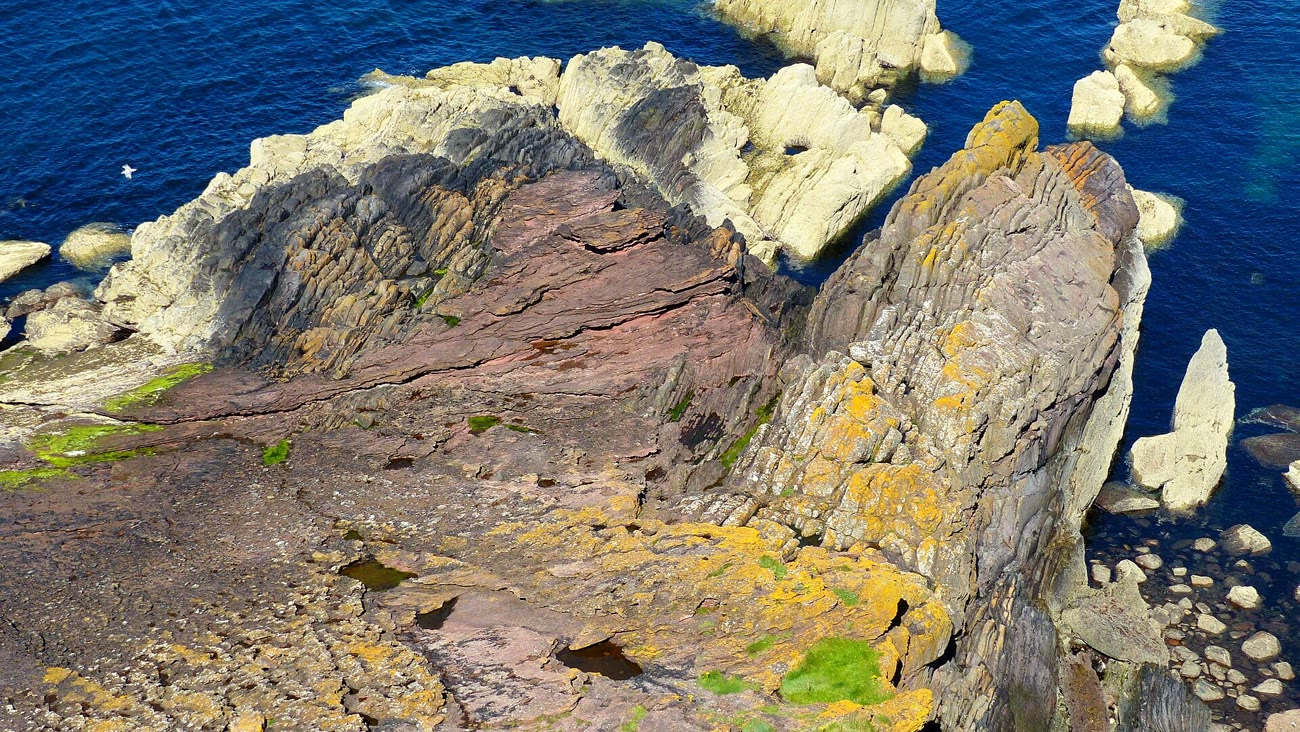
\includegraphics[width=0.7\linewidth]{images/book3/b1-siccar-point.jpg}

{\small Huttons \omterm{def:b1:cross-sections:unconformity}{discordantie} bij Siccar Point: bijna verticale grijze Siluurse lagen onderaan, licht hellende rode
Devoonse lagen erboven. Foto PawełS, CC BY-SA 4.0 (Wikimedia Commons).}
% ledger: commons:siccar-point
\end{center}
\end{history}

\begin{inthefield}[Geologie voor een tunnel]
\begin{minipage}[t]{0.6\linewidth}\vspace{0pt}
Voordat een tunnel wordt ontworpen, bouwen ingenieursgeologen doorsneden langs zijn lijn, uit de \omterm{def:b1:geological-maps:geological-map}{geologische
kaart}, uit boringen op regelmatige afstanden langs de route en uit geofysische metingen. Zij voorspellen elke eenheid
die de tunnel zal snijden, de breuken die hij zal kruisen en de plaatsen waar water kan binnenkomen. Tijdens het boren
registreren de geologen van de aannemer bij elke vordering het gesteente dat aan het front bloot komt, vergelijken dat
met de voorspelling en werken de doorsnede bij; proefboringen vooruit van de machine toetsen de grond voordat de machine
er komt, vooral nabij een voorspelde breuk of in kalksteen die holtes kan bevatten. Een breukzone van verbrijzeld
gesteente is een klassiek gevaar, des te meer wanneer hetzelfde gesteente aan beide kanten ligt en niets aan het front
waarschuwt.
\end{minipage}\hfill
\begin{minipage}[t]{0.37\linewidth}\vspace{0pt}
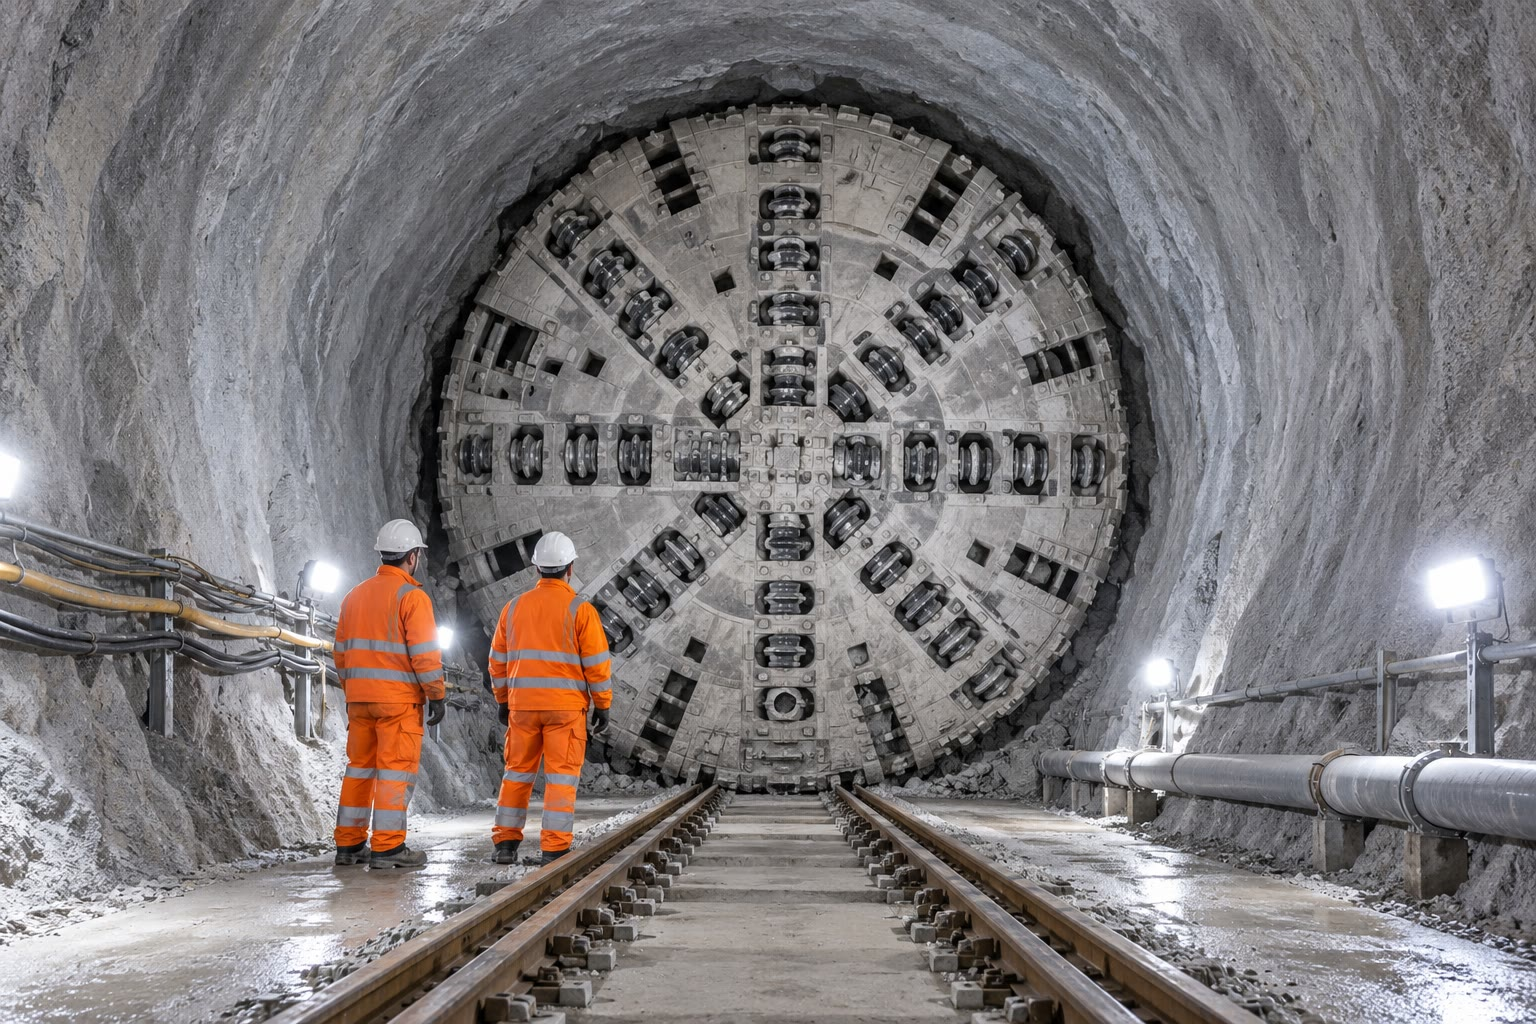
\includegraphics[width=\linewidth]{images/book3/ai/b1-tunnel-boring.jpg}
\end{minipage}
\end{inthefield}

\section{Oefeningen}

\begin{exercise}[$\star$]\label{exo:b1:cross-sections:1}
Een doorsnede wordt uit een kaart getekend op schaal 1:25\,000, met een verticale schaal van
\qty{1}{cm} per \qty{100}{m}. Wat is haar \omterm{def:b1:cross-sections:section}{verticale overdrijving}?
\end{exercise}

\begin{exercise}[$\star$]\label{exo:b1:cross-sections:2}
Een laag helt \ang{40} naar \ang{090}. Wat is haar \omterm{def:b1:cross-sections:apparent-dip}{schijnbare helling} in een verticale doorsnede met \omterm{def:b1:spherical-astronomy:horizontal}{azimut}
\ang{060}? Met \omterm{def:b1:spherical-astronomy:horizontal}{azimut} \ang{000}?
\end{exercise}

\begin{exercise}[$\star$]\label{exo:b1:cross-sections:3}
Een verticale boring snijdt \qty{120}{m} zandsteen waarvan de lagen onder \ang{12.16} helen. Wat is de \omterm{def:b1:cross-sections:thickness}{ware
dikte} van de zandsteen?
\end{exercise}

\begin{exercise}[$\star$]\label{exo:b1:cross-sections:4}
Een contact dat in het vlak van een doorsnede onder \ang{12} helt, wordt getekend met \omterm{def:b1:cross-sections:section}{verticale overdrijvingen}
van 2, 3 en 5. Onder welke hoeken verschijnt het?
\end{exercise}

\begin{exercise}[$\star\star$]\label{exo:b1:cross-sections:5}
Een laag helt \ang{25}. Haar \omterm{def:b1:geological-maps:geological-map}{ontsluiting} is \qty{300}{m} breed, loodrecht op de \omterm{def:b1:geological-maps:attitude}{strijk} gemeten. Bereken haar
\omterm{def:b1:cross-sections:thickness}{ware dikte} (a) op vlak terrein; (b) op terrein dat \ang{10} tegengesteld aan de helling helt, de breedte langs
het terrein gemeten; (c) op terrein dat \ang{10} in dezelfde richting als de helling helt.
\end{exercise}

\begin{exercise}[$\star\star$]\label{exo:b1:cross-sections:6}
Een laag toont in een noord--zuid doorsnede een \omterm{def:b1:cross-sections:apparent-dip}{schijnbare helling} van \ang{20} naar het noorden, en in een
oost--west doorsnede van \ang{30} naar het oosten. Bepaal haar \omterm{def:b1:geological-maps:attitude}{hellingrichting} en haar ware helling.
\end{exercise}

\begin{exercise}[$\star\star$]\label{exo:b1:cross-sections:7}
De basis van de kalksteen op de oostflank helt \ang{12.16}. Wat is de horizontale afstand van haar \omterm{def:b1:cross-sections:structure-contour}{structuurlijnen},
getekend om de \qty{100}{m}? Controleer dat op de \omterm{def:b1:cross-sections:structure-contour}{structuurlijnenkaart}.
\end{exercise}

\begin{exercise}[$\star\star$]\label{exo:b1:cross-sections:8}
Bereken uit de boringstabel de hoogte van de basis van de schalie in B1 en B3. Boven B2 is de schalie geërodeerd:
bereken uit de \omterm{def:b1:cross-sections:thickness}{verticale dikte} van de kalksteen de hoogte die haar basis daar zou hebben, en de \omterm{def:b1:cross-sections:apparent-dip}{schijnbare helling} van
dat contact tussen B1 en B2 in doorsnede C--D. Wat zegt de vergelijking van B1 en B3 over de \omterm{def:b1:geological-maps:fold}{plooi}?
\end{exercise}

\begin{exercise}[$\star\star$]\label{exo:b1:cross-sections:9}
Een normale breuk die \ang{50} naar \ang{180} helt, heeft een \omterm{def:b1:cross-sections:throw}{verticale verplaatsing} van \qty{150}{m}. Bereken
haar \omterm{def:b1:cross-sections:throw}{horizontale verplaatsing}. Wat zijn in een verticale doorsnede met \omterm{def:b1:spherical-astronomy:horizontal}{azimut} \ang{150} de \omterm{def:b1:cross-sections:apparent-dip}{schijnbare helling}
van de breuk en de afstand tussen de twee afsnijlijnen van een horizontale laag langs de doorsnede?
\end{exercise}

\begin{exercise}[$\star\star\star$]\label{exo:b1:cross-sections:10}
Voor een laag die \ang{40} helt: in welke richtingen van de doorsnede is de \omterm{def:b1:cross-sections:apparent-dip}{schijnbare helling} de helft van de ware
helling, dat wil zeggen \ang{20}? Toon aan dat de \omterm{def:b1:cross-sections:apparent-dip}{schijnbare helling} nabij de \omterm{def:b1:geological-maps:attitude}{hellingrichting} weinig en nabij de
\omterm{def:b1:geological-maps:attitude}{strijk} snel verandert.
\end{exercise}

\begin{exercise}[$\star\star\star$]\label{exo:b1:cross-sections:11}
Een boring snijdt de kalksteen van de oostflank (\omterm{def:b1:cross-sections:thickness}{ware dikte} \qty{176.0}{m}, helling \ang{12.16} naar \ang{080.7}).
Welke lengte kern levert zij op (a) als zij verticaal is; (b) als zij \ang{60} onder de horizontale naar \ang{260.7}
helt; (c) als zij \ang{60} naar \ang{080.7} helt? (Aanwijzing: de lengte is $t/\cos\psi$, waarin $\psi$ de hoek is
tussen de boring en de normaal op de gelaagdheid.)
\end{exercise}

\begin{exercise}[$\star\star\star$]\label{exo:b1:cross-sections:12}
Bij een \omterm{def:b1:cross-sections:unconformity}{hoekdiscordantie} helt de onderste laag \ang{70} naar \ang{090} en de bovenste laag \ang{20} naar
\ang{270}, met dezelfde \omterm{def:b1:geological-maps:attitude}{strijk}. Draai de hele \omterm{def:b1:geological-maps:geological-map}{ontsluiting} om de \omterm{def:b1:geological-maps:attitude}{strijk} tot de bovenste lagen weer horizontaal
liggen: wat was de helling van de onderste lagen toen de bovenste werden afgezet? Schrijf de geschiedenis van de
\omterm{def:b1:geological-maps:geological-map}{ontsluiting} in volgorde op.
\end{exercise}

\section{Probleem: Een tunnel onder de Varden Hills}

\begin{problem}[{Weekendprobleem --- welke gesteenten een tunnel zal snijden, waar hij de breuk ontmoet en hoeveel
kalksteen hij zal boren}]
\label{pb:b1:cross-sections:1}
% numbers from figdata/bachelor-1/varden_sections.py (model region.py) and the scratch calculator
De tunnel loopt recht naar het oosten langs de lijn C--D ($y = \qty{6}{km}$) op de constante hoogte van \qty{200}{m},
van $x = \qty{1}{km}$ tot $x =
\qty{9}{km}$. De grondhoogte langs C--D is, elke kilometer vanaf $x = 0$:
\begin{center}
\small
\begin{tabular}{lccccccccccc}
\hline
$x$ (km) & 0 & 1 & 2 & 3 & 4 & 5 & 6 & 7 & 8 & 9 & 10 \\
$z$ (m) & 509 & 556 & 467 & 370 & 435 & 534 & 501 & 455 & 406 & 339 & 405 \\
\hline
\end{tabular}
\end{center}
Gebruik de boringstabel van het hoofdstuk, de doorsnede C--D getekend met $e = 3$, de oriëntatie van de oostflank
(helling \ang{12.16} naar \ang{080.7}; de westflank is het spiegelbeeld, helling naar \ang{279.3}), en de normale breuk,
die \ang{60} naar \ang{120} helt, een \omterm{def:b1:cross-sections:throw}{verticale verplaatsing} van \qty{200}{m} heeft, en door het punt
$x = \qty{4.30}{km}$, $y = \qty{1.00}{km}$, $z = \qty{250}{m}$ gaat.

\medskip
\noindent\textbf{Deel I --- Het profiel en de eenheden.}
\begin{enumerate}
  \item Wat zijn de grootste en de kleinste diktes gesteente boven de tunnel op de kilometerpunten tussen
        $x = 1$ en $x = 9$?
  \item Op de afgedrukte doorsnede meet \qty{1}{km} horizontale afstand \qty{1.4}{cm} en meet \qty{1}{km} hoogte
        \qty{4.2}{cm}. Controleer dat $e = 3$.
  \item Vind in de \omterm{def:b1:cross-sections:log}{boorstaat} van B2 de hoogte van de basis van de zandsteen op de kruin van de \omterm{def:b1:geological-maps:fold}{antiklinaal}.
  \item In welke eenheid bevindt de tunnel zich bij $x = \qty{3.5}{km}$?
  \item Bereken de hoogte van de basis van de kalksteen in B1 en B3.
  \item Zet uit de doorsnede in volgorde de eenheden op een rij die de tunnel van $x = 1$ tot $x = \qty{9}{km}$ snijdt.
\end{enumerate}

\medskip
\noindent\textbf{Deel II --- Hellingen in de doorsnede.}
\begin{enumerate}[resume]
  \item Bereken de \omterm{def:b1:cross-sections:apparent-dip}{schijnbare helling} van de oostflank in C--D uit zijn oriëntatie.
  \item Controleer die uit de hoogten van de basis van de kalksteen in B2 en B3.
  \item Onder welke hoek is de oostflank in de doorsnede met $e = 3$ getekend?
  \item Bereken de \omterm{def:b1:cross-sections:apparent-dip}{schijnbare helling} van de breuk in C--D.
  \item Waarom ligt de \omterm{def:b1:cross-sections:apparent-dip}{schijnbare helling} van de poten in C--D zo dicht bij hun ware helling, en die van de breuk minder?
\end{enumerate}

\medskip
\noindent\textbf{Deel III --- De breuk.}
\begin{enumerate}[resume]
  \item Toon aan dat op het vlak $y = \qty{6}{km}$ de breuk ligt op
        \[ x = 4300 + \frac{2500 - (z - 250)\tan\ang{30}}{\sin\ang{120}}
           \quad\text{(meter)}. \]
  \item Waar ontmoet de tunnel de breuk?
  \item Bereken de \omterm{def:b1:cross-sections:throw}{horizontale verplaatsing} van de breuk, en de afstand tussen de afsnijlijnen van een contact langs C--D.
  \item Welk blok is omlaag bewogen, en welke eenheid ligt op tunnelhoogte aan elke kant van de breuk?
  \item Waarom is de breuk een gevaar dat de tunnelbouwers niet aan het front uit het gesteente konden zien aankomen?
        Hoe beschermen de ingenieurs zich ertegen?
\end{enumerate}

\medskip
\noindent\textbf{Deel IV --- De kalksteen.}
\begin{enumerate}[resume]
  \item Wat is de \omterm{def:b1:cross-sections:thickness}{verticale dikte} van de kalksteen in B1?
  \item Wat is haar \omterm{def:b1:cross-sections:thickness}{ware dikte}?
  \item Toon aan dat, west van de breuk op C--D, de basis van de zandsteen ligt op
        \[ z_b = 160.16 - |x - 3500|\tan\ang{12.0} \quad\text{(meter)}. \]
  \item De tunnel zit in de kalksteen wanneer zijn basis onder \qty{200}{m} ligt en zijn top erboven. Toon aan dat dit
        gebeurt voor $377.1 < |x - 3500|
        < 1224.0$.
  \item Geef de vier punten waar de tunnel de kalksteen binnenkomt en verlaat.
  \item Toon aan dat de lengte die op elke poot wordt geboord $h/\tan\beta$ is, waarin $h$ de \omterm{def:b1:cross-sections:thickness}{verticale dikte} is en
        $\beta$ de \omterm{def:b1:cross-sections:apparent-dip}{schijnbare helling}, en bereken haar.
  \item Welke totale lengte kalksteen boort de tunnel door?
\end{enumerate}
\end{problem}
